\documentclass[a4paper,10pt,twocolumn]{article}

\usepackage[header=false,
handles=false,
copydocumentclass=false,
active,
generate=2_rawtext.tex,
extract-env={document}]{extract}

%====================================PREAMBLE IMPORT====================================

%====================================ENCODING PACKAGES====================================
\usepackage[utf8]{inputenc}%
\usepackage[T1]{fontenc}%
\usepackage{textcomp}%
%====================================ENCODING PACKAGES====================================


%====================================FONT PACKAGES====================================
\usepackage{opensans}%
\usepackage{lmodern}%
%====================================FONT PACKAGES====================================


%====================================UTILITY PACKAGES====================================
\usepackage[english]{babel}%			--> english hyphenation, translation, etc for TeX stuff
\usepackage{csquotes}
\usepackage{import}
\usepackage{pdfpages}%				 	--> inserting .pdf files
\usepackage{amsmath}%				}
\usepackage{amssymb}%				}	--> math
\usepackage{geometry}%
\usepackage{graphicx}%
\usepackage{color}%
\usepackage{float}%
\usepackage{multicol}%					--> handling onecolumn figures
\usepackage{multirow}%				}
\usepackage{booktabs}%				}	--> nice tables
\usepackage{fancyhdr}%				 	--> nice headers
\usepackage{subfig}%					--> creation of subfloats for arrays of images
\usepackage[colorlinks=true,linkcolor=blue,citecolor=kekcolor]{hyperref}%
%====================================UTILITY PACKAGES====================================

%====================================PACKAGE RELATED CONFIGS====================================
\definecolor{kekcolor}{RGB}{15,163,59}
\definecolor{grun}{RGB}{0,127,0}
%\geometry{top=0.75 in, bottom=1in, left=0.75in, right=0.75in,columnsep=0.2in}%
\geometry{top=19mm, bottom=30mm, left=13mm, right=13mm,columnsep=4mm}%
%SOURCE ----> https://www.yumpu.com/en/document/read/48657545/preparation-of-papers-in-two-column-format-for-the-date
\setlength{\headheight}{14pt}%			--> fancyhdr requires a sufficent \headheight
\renewcommand{\arraystretch}{1.1}%		--> correcting for the look of tables (more room between each row)
%====================================PACKAGE RELATED CONFIGS====================================


%====================================GENERAL CONFIGS====================================
\setlength{\parindent}{0pt}%			--> no initial indents
\numberwithin{equation}{section}%		--> the equation counter loops in each succession of section counter
\makeatletter%						}
\@newctr{footnote}[section]%			} 	--> the footnote counter loops in each succession of the page counter
\makeatother%						}
%====================================GENERAL CONFIGS====================================


%====================================OBAMINA FAMILY OPERATORS====================================
\usepackage{obaminaandmore}%
%TexStudio may mark the used package as unkown. Ignore. It's in the folder as obamina_andmore.sty
%====================================OBAMINA FAMILY OPERATORS====================================


%=====================================STYLING THE SECTION TITLES====================================
\usepackage{titlesec}
\titleformat{\section}
{\fsi{12pt}\fsa{sc}\sefo}
{\fsi{13pt}\sefo\textbf{\thesection.}}
{2ex}
{\filcenter}


\titleformat{\subsection}
{\fsi{10pt}\fsa{sc}\sefo}
{\fsi{11pt}\sefo\textbf\thesubsection.}
{2ex}
{\filcenter  }
%====================================STYLING THE SECTION TITLES====================================


%====================================STYLING THE TABLE OF CONTENTS====================================
\usepackage{titletoc}
%\dottedcontents{section}[0pt]{}{2ex}{5cm}
\contentsmargin{1cm}
\titlecontents{section}[0pt]%format and left
			  {\addvspace{16pt}}% above-code
			  {\fse{b}\fsi{15pt}\os\sefo\thecontentslabel \hspace{2ex} }%numbered-entry-format
			  {\fse{b}\fsi{15pt}\os\sefo\thecontentslabel \hspace{2ex} }%numberless-entry-format
			  {\hfill {\fsi{14pt}\sefo \thecontentspage}}%filler-page-format
			  [\addvspace{4pt}]%below-code
			  
%\dottedcontents{subsection}[14ex]%format and left
%			   {\Large}%above-code alias global formatting of the entry
%			   {5ex}%label-width
%			   {5pt}%leader-with
			   
\titlecontents{subsection}[1cm]{}{\Large\thecontentslabel\hspace{3ex}}{\Large}{\hfill {\fsi{14pt}\sefo\thecontentspage}}
			  
%====================================STYLING THE TABLE OF CONTENTS====================================


%====================================FANCYHDR and HEADERS INIT====================================
\pagestyle{fancy}
\fancyhf{}
\renewcommand{\sectionmark}[1]{\markright{#1}}
\renewcommand{\subsectionmark}[1]{}
\fancyhead[LO]{\textbf {\fsi{11pt}\sefo \thesection}.\hspace{2ex}{\scshape \rightmark}}
\fancyhead[RO]{\textbf \thepage}
%====================================FANCYHDR and HEADERS INIT====================================


%====================================FONT COMMANDS====================================
\newcommand{\fsi}[1]{\fontsize{#1}{8pt}}
\newcommand{\fse}[1]{\fontseries{#1}}
\newcommand{\fsa}[1]{\fontshape{#1}}
\newcommand{\sefo}{\selectfont}
\newcommand{\os}{\fontfamily{opensans-TLF}}
\newcommand{\FT}{{\os\sefo FT}}
\newcommand{\IFT}{{\os\sefo IFT}}
%====================================FONT COMMANDS====================================


%====================================NEW COMMANDS====================================
\newcommand{\mypar}{\\[0.4\baselineskip]}
\newcommand{\BHJ}{{\os\sefo BHJ}}
\newcommand{\OSC}{{\os\sefo OSC}}
\newcommand{\BHSC}{{\os\sefo BHSC}}
%====================================NEW COMMANDS====================================


%====================================BIBLIOGRAPHY====================================
\usepackage[backend=biber,style=alphabetic,maxbibnames=10,maxcitenames=3]{biblatex}
%====================================BIBLIOGRAPHY====================================
%====================================PREAMBLE IMPORT====================================


%========================WE NEED LOCAL DEFINITION OF PATH TO BIB========================
\addbibresource{../../0_Bibliography/FPR.bib}
%========================WE NEED LOCAL DEFINITION OF PATH TO BIB========================


\begin{document}\begin{extract*}

\section{Characterization of the I-V-Curves}\label{sec:charac}

In order to characterize the assembled sets of \BHSC's, we used the Keithley~2602A~Sourcemeter and ABET~Technologies’ solar simulator SUN~2000. The simulator reproduces the AM 1.5 global reference spectrum and was also equipped with 5 different filters for varying the light intensity. Using the source meter we applied sequences of voltages to the cells and measured the currents resulting from their irradiation. This was done at different levels of intensity of light as well as darkness for which we covered each set with a plastic box.
\subsection{Irradiance calibration}
To ensure that the SUN~2000 was calibrated to yield an irradiance of $1\;\text{mW}\!\cdot\text{mm}^{-2}$, we used the Laser~Point PD-500-D9-VIS. With a digital caliper we measured the aperture of the photo diode to have a diameter of $d_p = 9.9(5)\;\text{mm}$. Here we had to assume such a high uncertainty because the construction of the aperture made it very difficult to make out the diameter. This yields an irradiated area of
\begin{equation*}
	A_p =  77(8)\;\text{mm}^2.
\end{equation*}
The total power $P_{p0}$ measured by the photo diode at maximum\footnote{This is the intensity corresponding to no filter. We will refer to it with the index 0.} intensity yielded $P_{p0} = 82(1)\;\text{mW}$. So that we arrive at an irradiance of
\begin{equation*}
	S_{p0} = 1.07(11)\;\frac{\text{mW}}{\text{mm}^2}.
\end{equation*}
As we will show in section~\ref{sec:broedelsec} there is external information (see \cite{photodiode}) on the aperture of the photo diode we could not make out at the time of the lab.
\begin{figure}[h]
	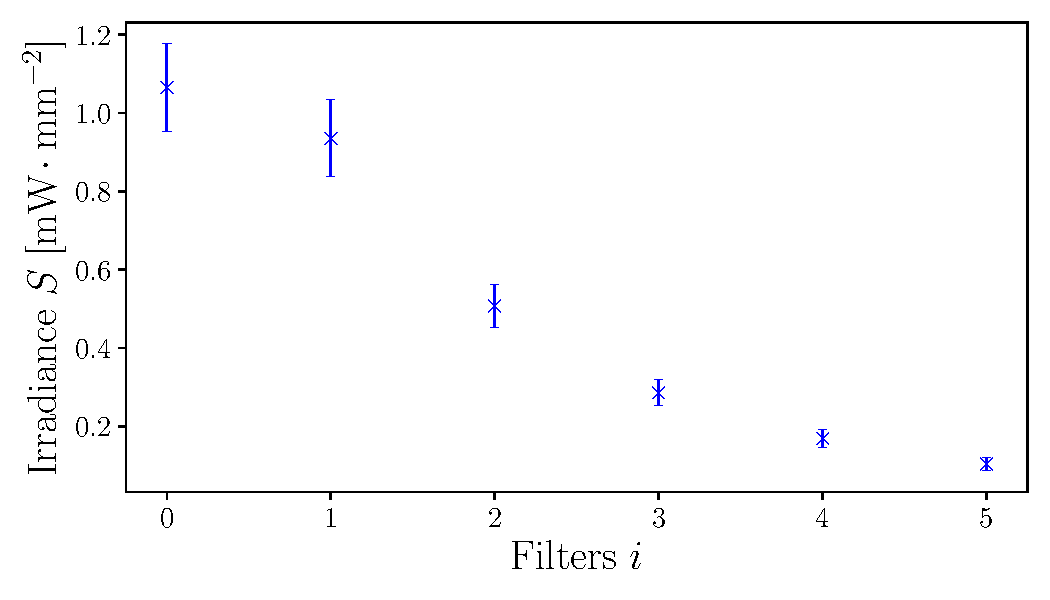
\includegraphics[scale=0.5]{../2_Pictures/Photodiode_irradiance.pdf}
	\caption{Measured irradiances $S_{pi}$ for each filter $i$ with Laser~Point PD-500-D9-VIS.}
	\label{fig:photodiode_irradiances}
\end{figure}

We also conducted this measurement with all filters available to us, in order to see how they modulate the intensity of the light. As we can deduct from figure~\ref{fig:photodiode_irradiances}, each filter does not modulate the lights intensity in a linear fashion. The relative decrease in irradiance from maximal to minimal light intensity is

\begin{equation}\label{eq:irrad-decrease}
	\Delta S = 1 - \frac{S_{p5}}{S_{p0}} \approx 90.2(19)\;\%.
\end{equation}
We were aware of the uncertainty in the measurements provided by the photo diode. Hence we performed additional measurements of I-V-curves using a Rera~RQN3686 silicon reference cell. This cell was calibrated on the AM 1.5 spectrum, so in order to check if our solar simulator was calibrated correctly we compared our measurements with the reference values (see \cite{reracat}) illustrated in table~\ref{tab:reracomp}. Because of no uncertainties given in the reference values, we are going to assume an error equal to a single unit in the last figure quoted (see \cite{measurements} section 2.8.1). For the determination of the uncertainty of our measured values we used the same methods as described in the section~\ref{subsec:calckeyparams} below. 
\begin{table}[h]\centering
	\caption{Comparison of our measurements with the reference values of the Rera~RQN3686 silicon reference cell for calibration purposes.}
	\label{tab:reracomp}
	\begin{tabular}{@{}lcc@{}}\toprule
		Quantity & Reference value & Measured value\\ \midrule
		$\jsc$ [mA$\cdot$cm$^{-2}$] & 32.7(1) & 32.783(16) \\
		$\Uoc$ [mV]& 596(1) & 596.3(4) \\ \bottomrule
	\end{tabular}
\end{table}

It is evident from table~\ref{tab:reracomp} that our measured results are deficient in accuracy but yield a better precision than those referenced. But nonetheless both of our measured values lie within the range of one $\sigma$ of the values specified by the manufacturer from which we conclude that the SUN~2000 was calibrated correctly.\mypar
Following the measurements depicted in figure~\ref{fig:photodiode_irradiances}, we investigated the performance of the silicon cell under the six different irradiances. We can see in figure~\ref{fig:reraPCE} that the power conversion efficiency with no filter present, reads $\eta_0 = 12.0(13)\;\%$. This deviates 22(9)~\% from the reference value (see \cite{reracat}). For the irradiance decrease in equation~\ref{eq:irrad-decrease} the silicon reference cells’ power conversion efficiency decreases by 50(10)~\%.
\begin{figure}[H]\centering
	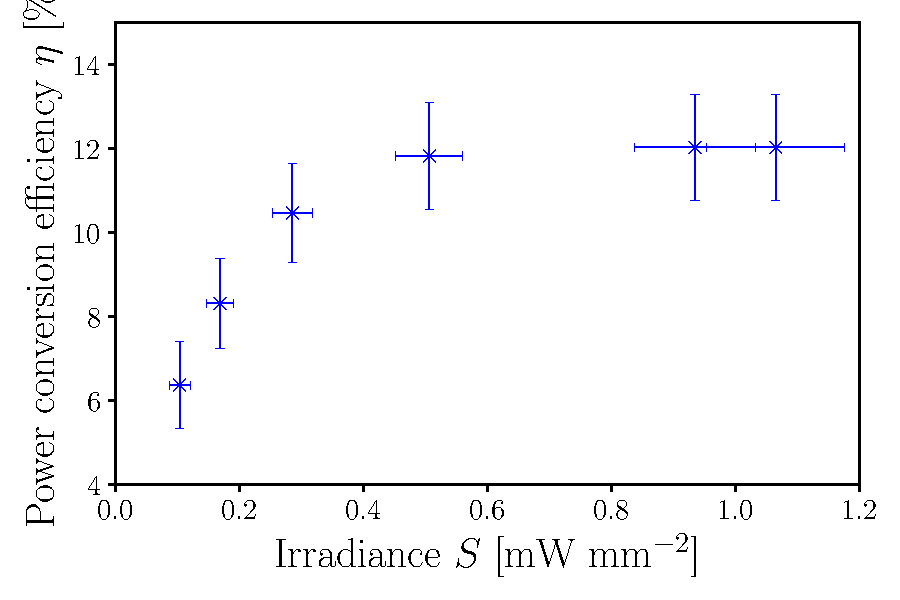
\includegraphics[scale=.5]{../2_Pictures/ReRaGraph.pdf}
	\caption{Power conversion efficiencies $\eta$ of the Rera~RQN3686 silicon reference cell.}
	\label{fig:reraPCE}
\end{figure}

\subsection{Calculation of key parameters}\label{subsec:calckeyparams}
In order to calculate the open circuit voltage $\Uoc$ and the short circuit current density $\jsc$ for a set of measurements, we performed a linear interpolation for each quantity. For each interpolation we used the two closest points to the relevant axis\footnote{Being the $j$-axis for $\Uoc$ and the $U$-axis for $\jsc$.} that were separated by it.\mypar
That means we will introduce two sets of points. For $\Uoc$ we choose $\{(j_1,U_1),(j_2,U_2)\}$ and for $\jsc$ we choose $\{(j_1^\prime,U_1^\prime),(j_2^\prime,U_2^\prime)\}$, for which the relationships for $\Uoc$ and $\jsc$ are 
\begin{align}\label{eq:interpol}
	\Uoc = \frac{U_2 j_1 - U_1 j_2}{j_1-j_2}\quad\text{and}\quad \jsc = \frac{U_1^\prime j_2^\prime - U_2^\prime j_1^\prime}{U_1^\prime-U_2^\prime}\;.
\end{align}
To get the maximum power density we simply multiplied all current densities and voltages and used the Python package \texttt{NumPy} to find the largest value.
\begin{align}
	\Pmax = \max_{i} (j_i\cdot U_i)
\end{align}
The fill factor $F\!F$ is defined as the ratio of maximum power to the product of $U_{\mathrm{OC}}$ and $j_{\mathrm{SC}}$.
\begin{align}
	F\!F = \frac{\Pmax}{\Uoc \cdot \jsc}
\end{align}
Finally the maximum power conversion efficiency $\eta$ is defined as the ratio of maximum power density to the irradiance of the incident light.
\begin{align}
	\eta = \frac{\Pmax}{S}
\end{align}

In the case of sets $\mathbb{S}_3$ and $\mathbb{S}_\star$ we had multiple working cells. For these we decided to do all calculations with the mean of the current density over the working cells $n$ on each set and include the standard error (see \cite{measurements} section 2.7) in the uncertainties of our results. The systematic errors of the current $u_{I,\text{sys}}$ and voltage $u_{U,\text{sys}}$ measurements were taken from \cite{keithley}. The uncertainty of the mean current density of measurement pair $p$ then is given as
\begin{equation}\label{eq:jerr}
	u_{\meann{j_p}} = \sqrt{\frac{\sigma_{j,p}^2}{N_\checkmark} + \meann{u_{j_p,\text{sys}}}^2} \;.
\end{equation}

With sample size $N_\checkmark$ being the amount of working cells of the set from table~\ref{tab:assemb-table}. The systematic error in equation~\ref{eq:jerr} results from Gaußian error propagation and thus reads
\begin{align}
	u_{j_{pn},\text{sys}} = \sqrt{ \left( \frac{ u_{I_{pn},\text{sys}}}{A_n}\right)^2+\left(j_{pn}\frac{u_{A_n}}{A_n} \right)^2}\;.
\end{align}

Uncertainties of all other expressions mentioned like equation~\ref{eq:interpol} are obtained through Gaußian error propagation.
\begin{figure}[H]\centering
	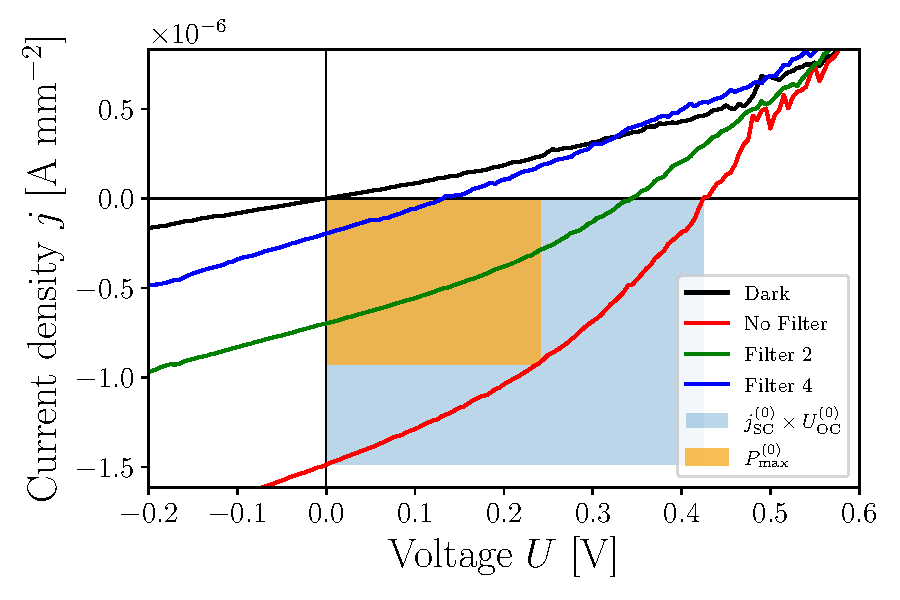
\includegraphics[width=\columnwidth]{../../../IV-Curve-Analysis/OSC1Graph.pdf}
	\caption{Current density measurements of set $\mathbb{S}_1$ for different light intensities. Blue depicts $U_{\mathrm{OC}}\!\cdot\!j_{\mathrm{SC}}$ and orange depicts $\Pmax$ for maximum light intensity.}
	\label{fig:OSC1Graph}
\end{figure}

\subsection{First set}\label{subsec:S1data}

In the following we will present the results of the sets $\mathbb{S}_1$, $\mathbb{S}_3$, $\mathbb{S}_5$ and $\mathbb{S}_\star$ which we acquired by performing the analysis described in the previous section.\mypar
For the first set $\mathbb{S}_1$ of \BHSC's, for which only one cell was not shorted, we obtained the following parameters in descending order of light intensity.
\begin{table}[H]\centering
	\caption{Overview of all obtained key parameters of set $\mathbb{S}_1$. Each row of the upper part of the table corresponds to the row in the lower half of the table. Depicted are all key parameters corresponding to each intensity.}
	\begin{tabular}{@{}cccc@{}}
		\toprule
		$\Pmax$ [\textmu $\text{W}\!\cdot\!\text{cm}^{-2}$] & $\jsc$ [\textmu A $\mathrm{cm}^{-2}$] & \multicolumn{1}{c}{$\Uoc$ [mV]} & $F\!F$ [\%] \\ \midrule
		$ 22.1(12) $                  & $ -149(5) $                           & \multicolumn{1}{c}{424.6(4)}    & 34.9(21)  \\
		$ 15.9(9) $                   & $ -124(4) $                           & \multicolumn{1}{c}{387.6(3)}    & 33.0(22)  \\
		$ 9.6(5) $                    & $ -70.0(24) $                         & \multicolumn{1}{c}{343.7(4)}    & 31.7(23)  \\
		$ 2.55(21) $                  & $ -37.0(13) $                         & \multicolumn{1}{c}{235.2(4)}    & 29.3(26)  \\
		$ 0.75(9) $                   & $ -19.7(7) $                          & \multicolumn{1}{c}{131.3(3)}    & 29(4)     \\
		$ 0.18(5) $                   & $ -10.5(4) $                          & \multicolumn{1}{c}{70.93(22)}   & 24(6)     \\ \midrule
		\multicolumn{2}{c}{$S_{i}$ [mW mm$^{-2}$]}                                               & \multicolumn{2}{c}{$\eta$ [\%]}             \\\midrule
		\multicolumn{2}{c}{1.06(11)}                                                              & \multicolumn{2}{c}{0.0207(24)}              \\
		\multicolumn{2}{c}{0.94(10)}                                                              & \multicolumn{2}{c}{0.0170(20)}              \\
		\multicolumn{2}{c}{0.51(5)}                                                               & \multicolumn{2}{c}{0.0151(19)}              \\
		\multicolumn{2}{c}{0.29(3)}                                                               & \multicolumn{2}{c}{0.0089(13)}              \\
		\multicolumn{2}{c}{0.169(22)}                                                             & \multicolumn{2}{c}{0.0045(8)}               \\
		\multicolumn{2}{c}{0.104(17)}                                                             & \multicolumn{2}{c}{0.0017(5)}               \\ \bottomrule
	\end{tabular}
\end{table}

In figure~\ref{fig:OSC1Graph} the current density measurements for four light intensities are shown. Similar to \cite{source1} we wanted to achieve a clear visualization for the key parameters. The blue rectangle indicates the product of short circuit current and open circuit voltage at the maximum intensity of light. The orange rectangle depicts the maximum power per area at maximum full intensity of incident light.
\begin{figure}[h]\centering
	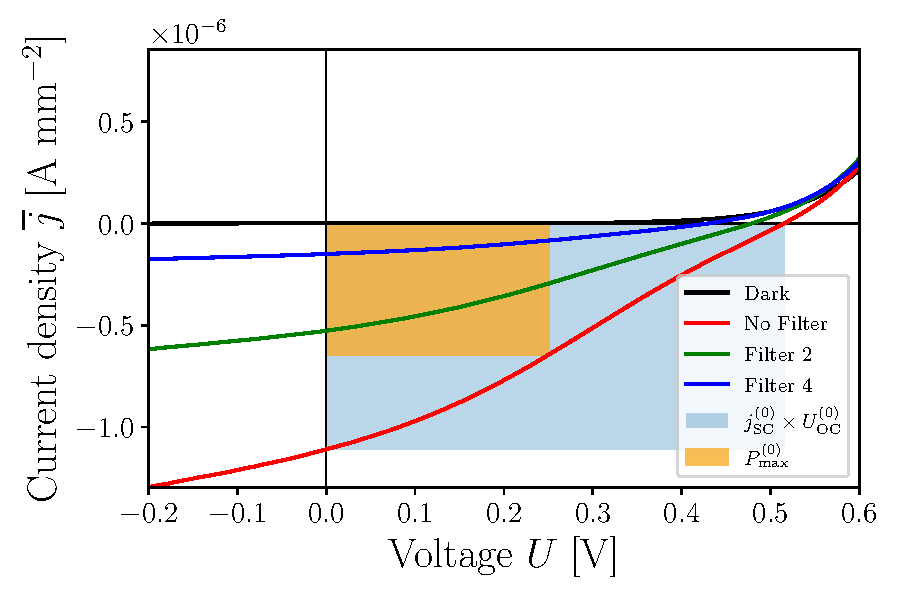
\includegraphics[width=\columnwidth]{../../../IV-Curve-Analysis/OSC2Graph.pdf}
	\caption{Current density measurements of set $\mathbb{S}_3$ for different light intensities.}
	\label{fig:OSC3Graph}
\end{figure}
\subsection{Third set}

We present the calculated key parameters for the third set of cells $\mathbb{S}_3$ analogously in figure~\ref{fig:OSC3Graph} and table~\ref{tab:OSC3table}. All cells on set $\mathbb{S}_3$ have the same architecture as set $\mathbb{S}_1$ (see table~\ref{tab:assemb-table}).

\begin{table}[h]
	\caption{Overview of all obtained key parameters of set $\mathbb{S}_3$. Each row of the upper part of the table corresponds to the row in the lower half of the table. Depicted are all key parameters corresponding to each intensity.}
	\label{tab:OSC3table}
	\begin{tabular}{@{}cccc@{}}
		\toprule
		$\Pmax$ [$\mu$W cm$^{-2}$] & $\jsc$ [$\mu$A $\mathrm{cm}^{-2}$] & $\Uoc$ [mV]     & $FF$ [\%]     \\ \midrule
		16.2(14)                   & -111(6)                            & 515(5)          & 28.2(29)      \\
		13.5(13)                   & -95(5)                             & 505(5)          & 28(3)         \\
		7.4(6)                     & -52.7(27)                          & 478.9(24)       & 29.3(29)      \\
		4.0(3)                     & -28.1(14)                          & 455.1(29)       & 31(3)         \\
		2.11(17)                   & -15.0(8)                           & 431.2(20)       & 33(3)         \\
		1.11(9)                    & -8.0(4)                            & 406.44(27)      & 34(3)         \\ \midrule
		\multicolumn{2}{c}{$S_p$ [mW mm$^{-2}$]}                        & \multicolumn{2}{c}{$\eta$ [\%]} \\ \midrule
		\multicolumn{2}{c}{1.06(11)}                                    & \multicolumn{2}{c}{0.0152(21)}  \\
		\multicolumn{2}{c}{0.94(10)}                                    & \multicolumn{2}{c}{0.0144(20)}  \\
		\multicolumn{2}{c}{0.51(5)}                                     & \multicolumn{2}{c}{0.0146(20)}  \\
		\multicolumn{2}{c}{0.29(3)}                                     & \multicolumn{2}{c}{0.0139(19)}  \\
		\multicolumn{2}{c}{0.169(22)}                                   & \multicolumn{2}{c}{0.0125(19)}  \\
		\multicolumn{2}{c}{0.104(17)}                                   & \multicolumn{2}{c}{0.0107(19)}  \\ \bottomrule
	\end{tabular}
\end{table}

\subsection{Preassembled set}

We did not measure the diameters $d_n^x$ and $d_n^y$ of the Galinstan droplets of the set $\mathbb{S}_\star$. In order to perform the analysis from section~\ref{subsec:calckeyparams} we used the average of all active areas $\langle A_{kn} \rangle$ from the cells of sets $\mathbb{S}_1$ and $\mathbb{S}_3$. We estimated the error in these areas to be the average uncertainty of said active areas $u_{A_\star} = \langle u_{A_{kn}}\rangle$ and found the results depicted in figure~\ref{fig:OSCstarGraph} and table~\ref{tab:OSCstartable}.

\begin{figure}[h]\centering
	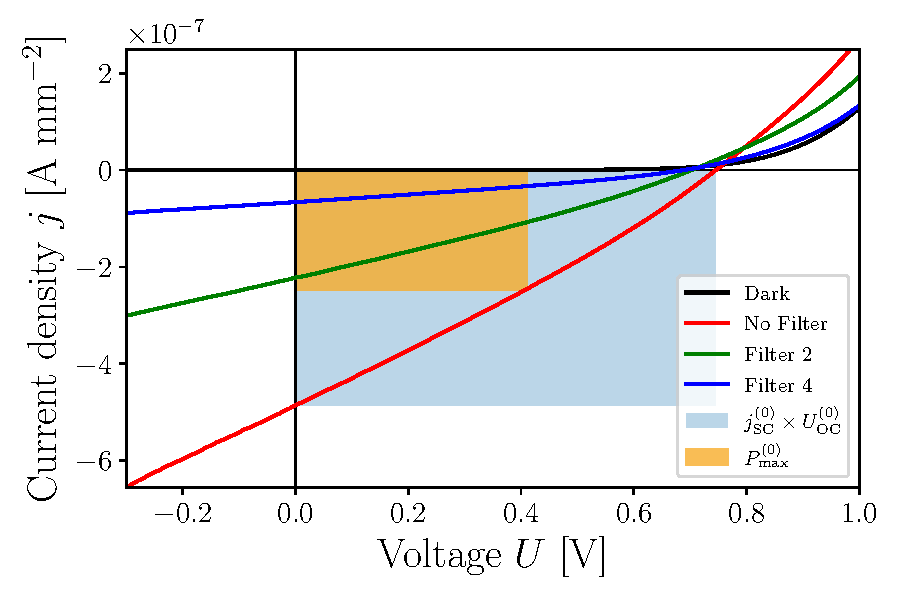
\includegraphics[width=\columnwidth]{../../../IV-Curve-Analysis/OSCPGraph.pdf}
	\caption{Current density measurements for the set $\mathbb{S}_\star$}
	\label{fig:OSCstarGraph}
\end{figure}

\begin{table}[h]
	\caption{Overview of all obtained key parameters of set $\mathbb{S}_\star$. Each row of the upper part of the table corresponds to the row in the lower half of the table. Depicted are all key parameters corresponding to each intensity.}
	\label{tab:OSCstartable}
	\begin{tabular}{@{}cccc@{}}
		\toprule
		$\Pmax$ [$\mu$W cm$^{-2}$] & $\jsc$ [$\mu$A $\mathrm{cm}^{-2}$] & $\Uoc$ [mV]          & $FF$ [\%]         \\ \midrule
		10.4(12)                   & -49(3)                             & 747(6)               & 28(3)             \\
		8.2(8)                     & -41.4(22)                          & 716(8)               & 27.7(29)          \\
		4.7(4)                     & -23.7(12)                          & 704(7)               & 28.4(29)          \\
		2.60(23)                   & -12.8(7)                           & 692(8)               & 29(3)             \\
		1.43(13)                   & -7.0(3)                            & 694(7)               & 30(3)             \\
		0.75(7)                    & -3.73(21)                          & 651(10)              & 31(4)             \\ \midrule
		\multicolumn{2}{c}{$S_p$ [mW mm$^{-2}$]}                        & \multicolumn{2}{c}{$\eta$ [\%]} \\ \midrule
		\multicolumn{2}{c}{1.06(11)}                                    & \multicolumn{2}{c}{0.0097(15)}           \\
		\multicolumn{2}{c}{0.94(10)}                                    & \multicolumn{2}{c}{0.0088(12)}           \\
		\multicolumn{2}{c}{0.51(5)}                                     & \multicolumn{2}{c}{0.0094(13)}           \\
		\multicolumn{2}{c}{0.29(3)}                                     & \multicolumn{2}{c}{0.0091(13)}           \\
		\multicolumn{2}{c}{0.169(22)}                                   & \multicolumn{2}{c}{0.0084(13)}           \\
		\multicolumn{2}{c}{0.104(17)}                                   & \multicolumn{2}{c}{0.0073(13)}           \\ \bottomrule
	\end{tabular}
\end{table}

\subsection{Special set}
We mentioned in section~\ref{subsec:lineupdesc} that the set $\mathbb{S}_5$ underwent a special treatment as we applied a PEIE layer instead of a PEDOT:PSS layer. Most of the $I$-$V$-curves of the cells of this set did not yield usable results, however by reversing the bias for one of the cells, we achieved a somewhat functional curve. It is illustrated in figure~\ref{fig:OSC5graph} with the numerical results contained in table~\ref{tab:OSC5table}.
\begin{figure}[h]
	\centering
	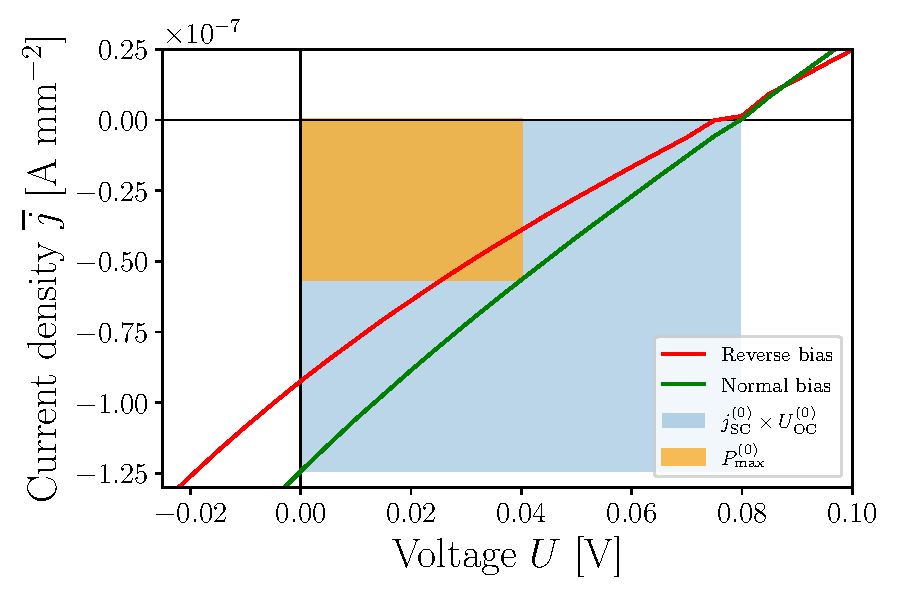
\includegraphics[width=\columnwidth]{../../../IV-Curve-Analysis/OSC5Graph.pdf}
	\caption{Current density measurement for set $\mathbb{S}_5$ at full intensity after reversing the bias}
	\label{fig:OSC5graph}
\end{figure}

\begin{table}[h]
	\centering
	\caption{Overview of all obtained key parameters of set $\mathbb{S}_5$. These measurements were done without a filter in front of the solar simulator.}
	\label{tab:OSC5table}
	\begin{tabular}{@{}lc@{}}
		\toprule
		 Quantity&Value\\\midrule 
		$\Pmax$ [$\mu$W cm$^{-2}$] & 0.16(7) \\
		$\jsc$ [$\mu$A $\mathrm{cm}^{-2}$]             & -9.2(3)                     \\ 
		$\Uoc$ [mV]                                    & 75.58(24)                   \\
		$FF$ [\%]                                      & 22(10)                      \\ 
		$\eta$ [\%]                                    & 15(6)$\cdot 10^{-5}$                  \\ \bottomrule
	\end{tabular}
\end{table}
\end{extract*}
\end{document}